\chapter{\textit{Introdução}}

O desenvolvimento de veículos aéreos não tripulados (VANTs), ou popularmente conhecido como drones, tem ganhado uma atenção maior nas últimas décadas principalmente em aplicações militares. As configurações mais comuns de drone são os quadricópteros, devido sua habilidade de pairar silenciosamente a baixas altitudes, acelerar rapidamente e alterar sua orientação conforme necessário. Essas características fazem dele uma excelente escolha para drones de pequeno porte (KADHIM; ABDULSADDA, 2020). Assim, dentro dessa categoria, os quadricópteros com seus rotores dispostos em configuração simétrica são os mais comuns, devido à sua simplicidade de design e eficiência no controle do movimento.

\begin{figure}[H]
	\centering
	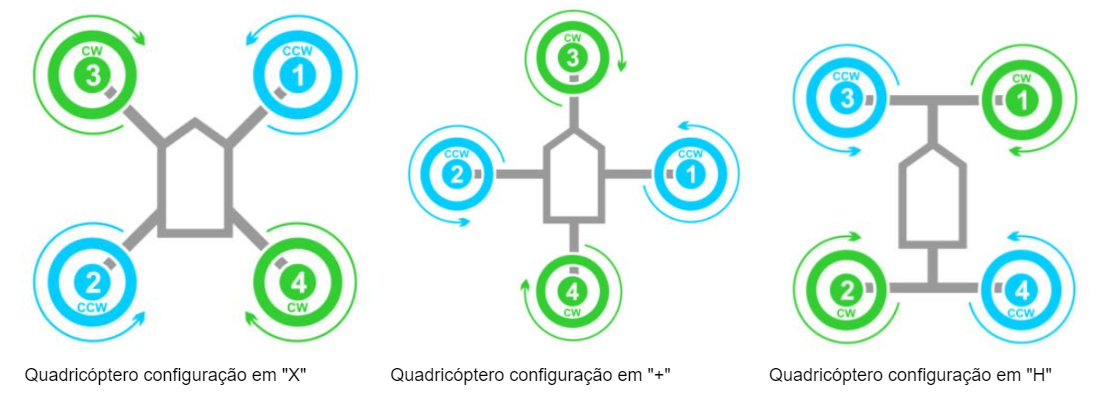
\includegraphics[width=0.6\textwidth]{possible_configs_quadcopter.png}
	\caption{Quadricópteros com rotores em configuração simétrica.}
	\centering
	\label{multiple drone rotor configuration}
\end{figure}


Com o passar do tempo, além das aplicações militares, os drones passaram a ter também uso recreativo, seja simplesmente para pilotar o drone, para tirar fotos, ou até mesmo situações mais complexas como seguir uma trajetória pré-determinada. Hoje, além do uso recreativo os quadricópteros se tornaram plataformas interessantes para pesquisa científica e desenvolvimento de soluções para engenharia de controle.  Pelo seu tamanho compacto e sua característica de sistema subatuado, ou seja, com menos atuadores do que graus de liberdade, os quadricópteros são suscetíveis a muitas incertezas e turbulências, como rajadas de vento, mudanças climáticas, entre outros,
sendo que a complexidade de sua dinâmica e o acoplamento não linear entre os graus de liberdade do sistema, fazem com que o estudo e o controle desse tipo de drone sejam áreas de interesse contínuo que desafiam os engenheiros e pesquisadores a desenvolver controles eficazes que garantam a estabilidade e o desempenho desejado em condições adversas.

Nesse cenário, este trabalho se dedica à análise dinâmica e de controle de um mini drone específico: o Parrot Mambo. Este modelo foi escolhido, pois tem-se mostrado uma excelente plataforma para fins educacionais e de pesquisa, devido à sua acessibilidade e à sua facilidade de integração com ferramentas de simulação, como o MATLAB Simulink. De acordo com a MathWorks (2024), o Parrot Mambo pode ser amplamente utilizado em experimentos acadêmicos, principalmente em estudos de controle, por oferecer um exemplo prático de um quadricóptero com um sistema de controle embarcado que pode ser testado e simulado em ambiente virtual.

\begin{figure}[H]
	\centering
	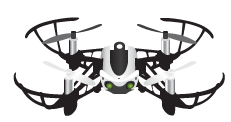
\includegraphics[width=0.5\textwidth]{parrot_mambo_stabilized.png}
	\caption{Drone Parrot Mambo utilizado nesse trabalho}
	\centering
	\label{drone-parrot}
\end{figure}


Tendo em vista essa possibilidade, utilizaremos o modelo de controle disponibilizado pela Parrot em parceria com a MathWorks, que permite que possamos explorar os algoritmos já desenvolvidos e propor melhorias, quando necessário e possível. Logo, o principal objetivo deste trabalho é analisar a dinâmica e avaliar o sistema de controle do quadricóptero, assim, para facilitar as simulações será utilizado o bloco 6DOF (Ângulos de Euler) no MATLAB Simulink para modelar as equações de movimento com base nos 6 graus de liberdade (três de translação e três de rotação), embora utilizemos um bloco pronto para as simulações, uma seção específica do trabalho será dedicada para explicar detalhadamente como as equações de movimento que descrevem esses graus de liberdade são obtidas. Esse processo incluirá a análise da cinemática e dinâmica do quadricóptero, com base nos ângulos de Euler para descrever as rotações e nas leis de Newton-Euler para modelar a translação e rotação do sistema. Serão abordados os conceitos de forças e momentos atuantes no drone, bem como o acoplamento entre os diferentes graus de liberdade, proporcionando uma base teórica sólida para o entendimento da simulação MATLAB Simulink. Assim, a simulação vai nos permitir analisar o desempenho dos controladores clássicos utilizados, como o Proporcional-Integral-Derivativo (PID), e a partir dessa análise, será possível identificar os parâmetros mais importantes do sistema e possivelmente propor ajustes ou otimizações que melhorem o comportamento do drone em simulações.

Além disso, o trabalho se propõe a analisar os resultados obtidos através das simulações no MATLAB Simulink. As simulações permitirão a avaliação do desempenho do controlador atual e a identificação de possíveis pontos de melhoria com base no comportamento observado. Embora não seja o foco deste trabalho realizar os testes no drone físico, o ambiente de simulação poderá proporcionar uma visão detalhada do desempenho do sistema de controle. Este estudo busca não somente aprimorar o sistema de controle do Parrot Mambo no contexto da simulação, mas também contribuir para um entendimento mais profundo da dinâmica e das técnicas de controle aplicáveis aos quadricópteros.







%---------------------------------------------------------------------
% INDICE REMISSIVO
%---------------------------------------------------------------------
\phantompart
\printindex
%---------------------------------------------------------------------
